\documentclass[aspectratio=169, pdf, 8pt, unicode]{beamer}
\usepackage[american,russian]{babel}
\usepackage[default]{sourcesanspro}
\usepackage{float}
\usepackage{graphicx}
\usepackage{pgfplotstable}
\usepackage{caption}
\usepackage{amsmath}
\usepackage{amssymb}
\usepackage{setspace}
\usepackage{fancyvrb}
\usepackage[outputdir=aux]{minted}
\usepackage{url}

\DeclareCaptionLabelFormat{gostfigure}{Рисунок #2}
\captionsetup[table]{labelsep=endash,justification=justified,singlelinecheck=false,font=normalsize,skip=0pt} 
\captionsetup[figure]{labelformat=gostfigure,labelsep=endash,justification=centering,singlelinecheck=false,font=normalsize} 
\pgfplotsset{compat=1.9}

\mode<presentation> {
\usetheme{Madrid}
}

\setbeamerfont{institute}{size=\normalsize}
\setbeamertemplate{itemize/enumerate body begin}{\large}
\setbeamertemplate{itemize/enumerate subbody begin}{\tiny}

\title[Теория и практика многопоточного программирования]{Теория и практика многопоточного программирования}

\author{Неганов Алексей}

\institute[МФТИ]{
    Московский физико-технический институт (национальный исследовательский университет)\\
    Кафедра теоретической и прикладной информатики\\
}

\date{Москва 2020}

\setbeamertemplate{caption}[numbered]

\begin{document}

\begin{frame}
\titlepage
\end{frame}

\begin{frame}[fragile]
\frametitle{C10K problem}
\begin{figure}[H]
      \centering
      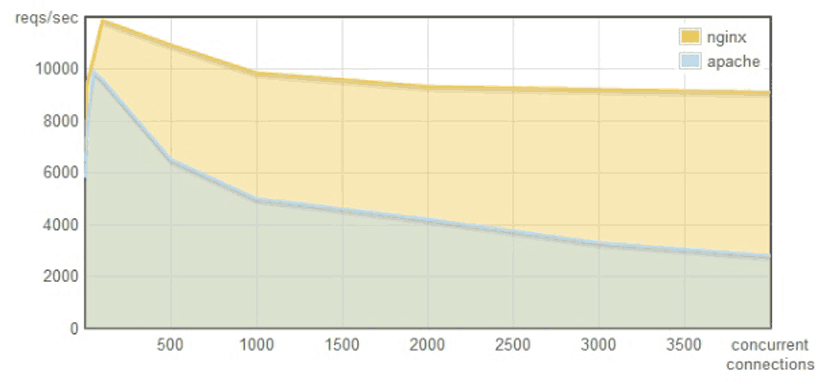
\includegraphics[width=0.6\textwidth]{fig/nginx-apache-10kreqs.png}
      \caption{Сравнение поведения веб-серверов Nginx и Apache при увеличении количества обновременных подключений}
\end{figure}
\end{frame}

\begin{frame}[fragile]
\frametitle{Green threads / goroutines}
\begin{figure}[H]
      \centering
		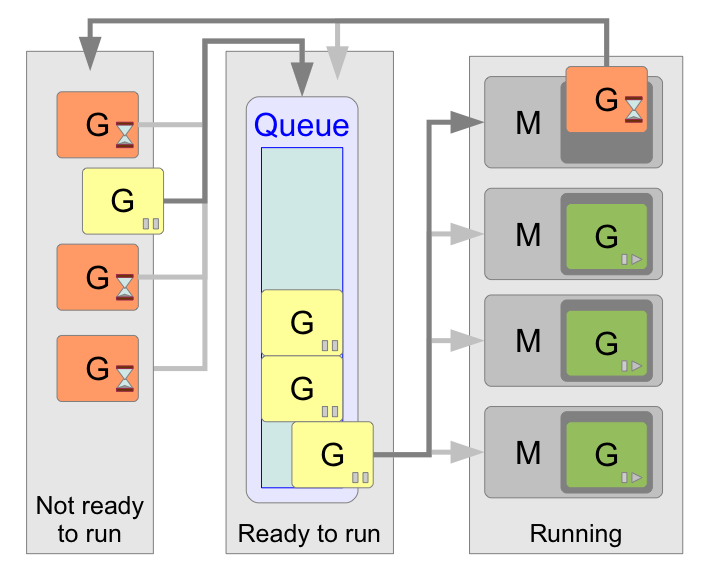
\includegraphics[width=0.55\textwidth]{fig/goroutines.png}
      \caption{Схема работы планировщика Go}
\end{figure}
\end{frame}

\begin{frame}[fragile]
\frametitle{Worker pool}
\begin{figure}[H]
\centering
\begin{minipage}{0.5\textwidth}
\small
\begin{minted}{Go}
package main

import (
    "fmt"
    "time"
)

func worker(id int, jobs <-chan int, results chan<- int) {
    for j := range jobs {
        fmt.Println("worker", id, "started  job", j)
        time.Sleep(time.Second)
        fmt.Println("worker", id, "finished job", j)
        results <- j * 2
    }
}
\end{minted}
\end{minipage}%
\begin{minipage}{0.4\textwidth}
\small
\begin{minted}{Go}
func main() {
    const numJobs = 5
    jobs := make(chan int, numJobs)
    results := make(chan int, numJobs)

    for w := 1; w <= 3; w++ {
        go worker(w, jobs, results)
    }

    for j := 1; j <= numJobs; j++ {
        jobs <- j
    }
    close(jobs)

    for a := 1; a <= numJobs; a++ {
        <-results
    }
}
\end{minted}
\end{minipage}
\end{figure}
\begin{itemize}
\item Входная очередь
\item Выходная очередь / мультиплексирование
\end{itemize}
\end{frame}

\begin{frame}
\frametitle{Worker pool}
\begin{figure}[H]
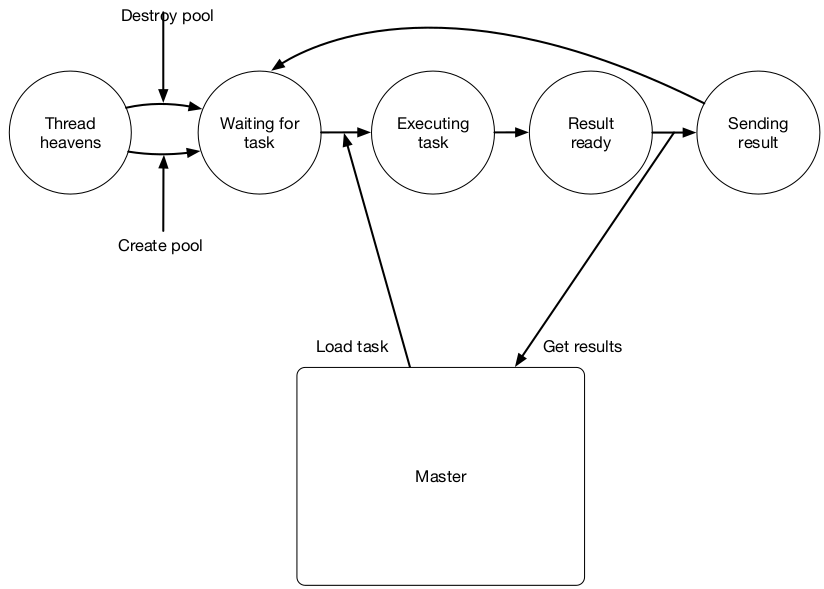
\includegraphics[width=0.7\textwidth]{fig/thread-pool-states.png}
\end{figure}
\end{frame}

\begin{frame}
\frametitle{Worker pool}
\begin{figure}[H]
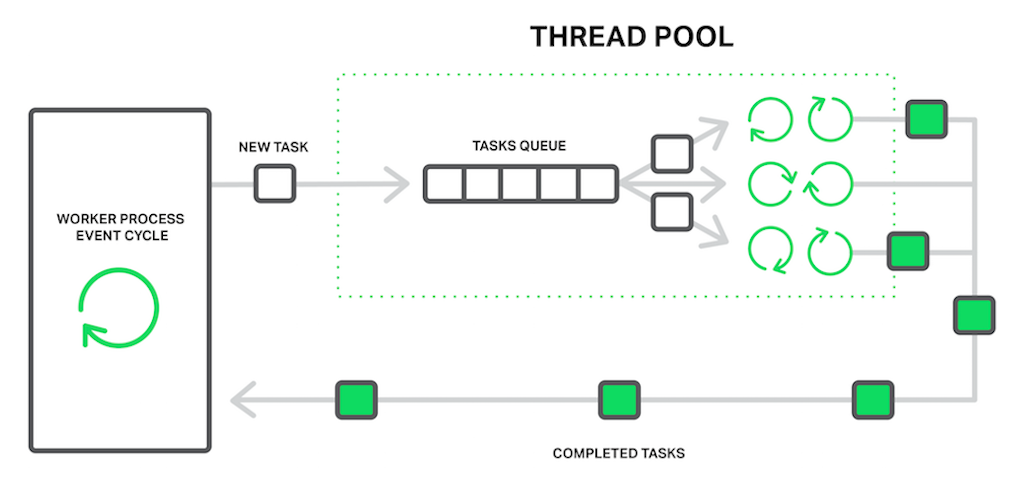
\includegraphics[width=0.8\textwidth]{fig/thread-pools-worker-process-event-cycle.png}
\end{figure}
\end{frame}

\begin{frame}
\frametitle{Work stealing}
\begin{figure}[H]
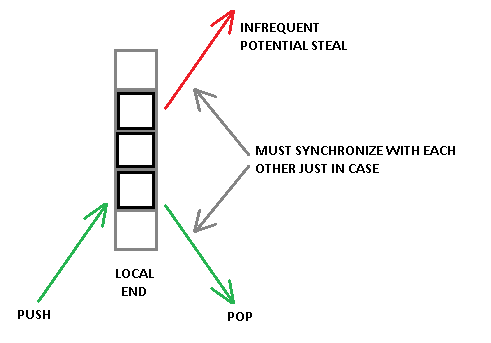
\includegraphics[width=0.6\textwidth]{fig/stealing.png}
\end{figure}
\end{frame}

\end{document}
